%%%%%%%%%%%%%%%%%%%%%%%%%%%%%%%%%%%%%%%%%%%%%%%%%%%%%%%%%%%%%%%%%%%%%%%%%%%%%%%
%                         File: osa-revtex4-1.tex                             %
%                        Date: April 15, 2013                                 %
%                                                                             %
%                              BETA VERSION!                                  %
%                   JOSA A, JOSA B, Applied Optics, Optics Letters            %
%                                                                             %
%            This file requires the substyle file osajnl4-1.rtx,              %
%                   running under REVTeX 4.1 and LaTeX 2e                     %
%                                                                             %
%                   USE THE FOLLOWING REVTeX 4-1 OPTIONS:                     %
% \documentclass[osajnl,twocolumn,showpacs,superscriptaddress,10pt]{revtex4-1}%
%                    %% Use 11pt for Applied Optics                           %
%                                                                             %
%               (c) 2013 The Optical Society of America                       %
%                                                                             %
%%%%%%%%%%%%%%%%%%%%%%%%%%%%%%%%%%%%%%%%%%%%%%%%%%%%%%%%%%%%%%%%%%%%%%%%%%%%%%%

\documentclass[osajnl,twocolumn,showpacs,superscriptaddress,10pt]{revtex4-1} %% use 10pt for Applied Optics
%%\documentclass[osajnl,preprint,showpacs,superscriptaddress,12pt]{revtex4-1} %% use 12pt for preprint option
\usepackage{amsmath,amssymb,graphicx,float,enumerate}
\usepackage[cache=false]{minted}
\usepackage[utf8]{inputenc}
\graphicspath{ {../images/} }

\usepackage[colorlinks = true,
            linkcolor = black,
            urlcolor  = blue,
            citecolor = black,
            anchorcolor = blue]{hyperref}

\usepackage{silence}
\WarningFilter{revtex4-1}{Repair the float}

\begin{document}

\title{Redes y Comunicaciones}

\author{Ulises Jeremias Cornejo Fandos}
\affiliation{13566/7, Licenciatura en Informatica, Facultad de Informatica, UNLP}

\author{Federico Ramón Gasquez}
\affiliation{13598/6, Licenciatura en Informatica, Facultad de Informatica, UNLP}

\author{Lihuel Pablo Amoroso}
\affiliation{13497/2, Analista Programador Universitario, Facultad de Informatica, UNLP}

%%\begin{abstract}
%%\end{abstract}

\maketitle %% required

\onecolumngrid

\section{Ejercicio 1}

\textit{Utilizando topología topologia-IP.imn y dado el bloque IPv6: 2001:db8:1234::/48.}

\begin{enumerate}[a)]
    \item Arme el plan de direccionamiento IPv6 teniendo en cuenta las siguientes restricciones:
    
    \begin{itemize}
        \item La red A tiene 70 hosts y se espera un crecimiento máximo de 20 hosts.
        \item La red X tiene 150 hosts.
        \item La red B cuenta con 20 hosts
        \item La red Y tiene 35 hosts y se espera un crecimiento máximo de 30 hosts.
        \item Los bloques IP asignados en los enlaces entre routers podrán ajustarse a desperdiciar pocas direcciones.
        \item Es importante utilizar VLSM?
    \end{itemize}

    \item Asigne direcciones IP en los equipos de la topología según el plan anterior.
    \item Configure las tablas de rutas teniendo en cuenta las siguientes restricciones:
    \item n1 deberá optar por el enlace verde solamente para rutear el tráfico dirigido a la Red X.
    \item Utilizando la herramienta ping6(8), verifique conectividad entre los hosts pertenecientes a las diferentes redes de usuarios.
\end{enumerate}

Se adjunta el archivo \textit{resources/topologia.imn} en la cual se encuentra la topologia de la red diseñada
cumpliendo todos los requisitos. En la misma no solo se encuentran las asignaciones de IPv6, sino también las
IPv4 correspondientes al último enunciado. \\

Para armar el plan de direccionamiento IPv6 de esta topologia no es necesario utilizar VLSM dado que
la cantidad de host a asignar por red nunca llegan a ser tantas como para que no alcanse la cantidad
de IPs asignables.

\section{Ejercicio 2}

\textit{TTL (Adjunte capturas de tráfico para cada uno de los incisos).}

\begin{enumerate}[a)]
    \item \textit{Utilizando el comando \textbf{traceroute6/tracepath6(8)}, realice una
    traza entre el host n8 y n10, tanto utilizando UDP como ICMP.
    ¿Qué diferencias tiene cada método y en qué casos utilizaría cada
    uno?.} \\

    El comando \textbf{traceroute6} envia en ambos casos, utilizando tanto UDP como ICMP,
    un paquete con el valor del campo TTL \textit{(time to live)} de la cabecera IP igual a 1,
    esperando una respuesta ICMP de la forma \textit{Time Exceeded} ó \textit{Time to Live Expired} del primer router que recibe
    el mensaje, ya que en el primer salto el TTL se habrá decrementado a 0. Luego se incrementa el TTL en 1, 
    esperando recibir una respuesta del segundo router involucrado, y se repite el proceso para construir el camino hasta 
    recibir una respuesta del destino al que se quería conocer inicialmente. \\

    La diferencia radica en que, bajo el protocolo ICMP, se envian paquetes del tipo \textit{echo request} esperando que, 
    una vez que se llegue al destino, este último envie un \textit{echo reply}. El problema es que puede que algunos 
    routers filtren los mensajes de tipo echo request, imposibilitando encontrar a través de este protocolo la ruta completa; 
    en este caso conviene realizar el traceroute a través de UDP. Este último envía mensajes de tipo UDP a un puerto destino 
    válido, y una vez que llega al router destino, este le enviara un mensaje indicando que el puerto destino es inalcanzable.

    \begin{figure}[H]
        \centering
        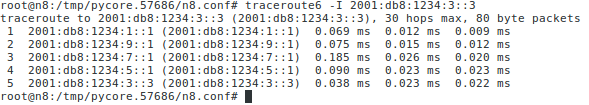
\includegraphics[width=0.75\textwidth]{traceroute6icmp.png}
        \caption{Traza entre el comando n8 y n10 utilizando traceroute6 con ICMP.}
        \label{image:traceroute6icmp}
    \end{figure}

    \begin{figure}[H]
        \centering
        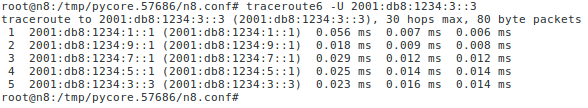
\includegraphics[width=0.75\textwidth]{traceroute6udp.png}
        \caption{Traza entre el comando n8 y n10 utilizando traceroute6 con UDP.}
        \label{image:traceroute6udp}
    \end{figure}

    Se adjunta el tráfico captura en los archivos \textit{resources/traceroute6icmp.pcapng} y \textit{resources/traceroute6ucp.pcapng}. \\

    \item \textit{Realice un ping entre n8 y n5 y determine el valor inicial del
    campo TTL capturando tráfico en la interfaz eth0 del host n8.}

    Para este inciso, se ejecuta en la terminal correspondiente al host n8 un ping entre este host y n7
    utilizando el comando \textit{ping6}. \\

    Capturando el tráfico con el wireshark se busca determinar el valor del campo TTL en
    el header del paquete IPv6. Tras no poder encontrarlo se inspecciona el formato de una
    cabecera IPv6 y concluyendo que dicha información se puede obtener en el header Hop Limit. 
    Leer \href{https://tools.ietf.org/html/rfc2460}{RFC 2460}. \\

    Se puede observar entonces en la figura \ref{image:ttl}, que el valor inicial
    del campo TTL, \textit{Hop Limit en IPv6}, es 64 en la interfaz eth0 del host n8.

    \begin{figure}[H]
        \centering
        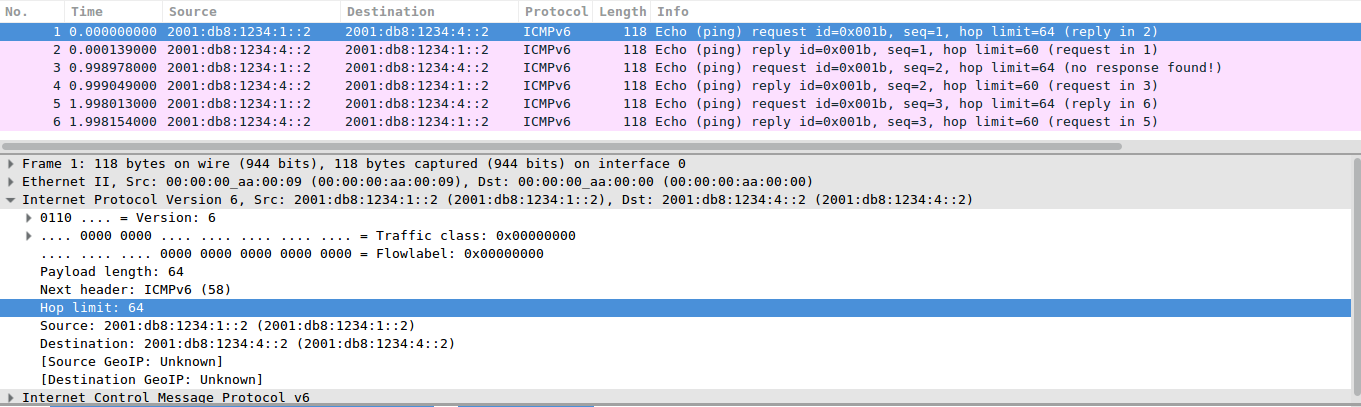
\includegraphics[width=0.95\textwidth]{ttl.png}
        \caption{Captura del tráfico del ping entre n8 y n7 en el que se observa el valor inicial del campo Hop Limit.}
        \label{image:ttl}
    \end{figure}

    \item \textit{A través de la capturas de tráfico, determine en qué momento el
    router decrementa el valor del TTL.}

    Dada la ejecución del comando presentado en la figura \ref{image:ping6-n8-n7} se pueden apreciar las capturas de paquetes de cada 
    uno de los routers en las figuras \ref{image:tcpdump-n1}, \ref{image:tcpdump-n11}, \ref{image:tcpdump-n6} y \ref{image:tcpdump-n3}.

    \begin{figure}[H]
        \centering
        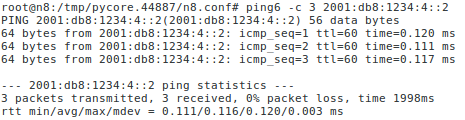
\includegraphics[width=0.75\textwidth]{ping6-n8-n7.png}
        \caption{Salida de la ejecución del comando ping realizado del nodo n8 al n7.}
        \label{image:ping6-n8-n7}
    \end{figure}

    Observando las capturas de la interfaz de salida de cada uno de los routers a través de los cuales viaja el ping, 
    se ve como el TTL, \textit{Hop Limit} en IPv6, se decrementa con respecto a la captura del mismo router en la interfaz 
    de entrada del mensaje, es decir, que el router lo decrementa previo al forwarding. \\

    \begin{figure}[H]
        \centering
        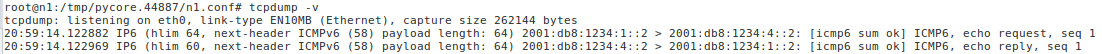
\includegraphics[width=0.95\textwidth]{tcpdump-n1.png}
        \caption{Captura realizada desde el router n1 del tráfico entre n8 y n7.}
        \label{image:tcpdump-n1}
    \end{figure}

    \begin{figure}[H]
        \centering
        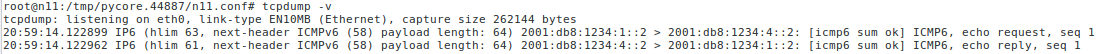
\includegraphics[width=0.95\textwidth]{tcpdump-n11.png}
        \caption{Captura realizada desde el router n11 del tráfico entre n8 y n7.}
        \label{image:tcpdump-n11}
    \end{figure}

    \begin{figure}[H]
        \centering
        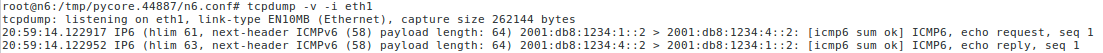
\includegraphics[width=0.95\textwidth]{tcpdump-n6.png}
        \caption{Captura realizada desde el router n6 del tráfico entre n8 y n7.}
        \label{image:tcpdump-n6}
    \end{figure}

    \begin{figure}[H]
        \centering
        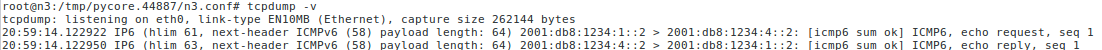
\includegraphics[width=0.95\textwidth]{tcpdump-n3.png}
        \caption{Captura realizada desde el router n3 del tráfico entre n8 y n7.}
        \label{image:tcpdump-n3}
    \end{figure}

    \item \textit{Utilizando la herramienta para enviar mensajes ICMP con la opción
    -t desde n8 envíe un datagrama a n7 con TTL=1. ¿Qué mensaje recibe? ¿Por qué?}

    Para enviar mensajes ICMP se utiliza el comando ping(6) ejecutando, en la 
    terminal del nodo n8, el siguiente comando,

    \begin{minted}{bash}
        $ ping6 -t 2001:db8:1234:4::2
    \end{minted}

    , siendo 2001:db8:1234:4::2 la IPv6 del nodo n7. \\

    A la par que se envía el datagrama, se captura el tráfico utilizando wireshark
    como se observa en la figura (\ref{image:ttl1}). El mensaje que se recibe tanto en la
    salida del comando ejecutado (figura \ref{image:ttl1ping}) como en los paquetes
    capturados por el wireshark es \textit{Time exceeded: Hop Limit}. \\

    Dado que el valor inicial del TTL es 1, el primer salto cuando va hacia el primer router de la red, 
    decrementa el TTL, llevando su valor a 0 y en consecuencia, descartando el paquete, posteriormente 
    le envía un mensaje ICMP al host indicándole que se excedió el tiempo del TTL, \textit{Time exceeded: Hop Limit}.

    \begin{figure}[H]
        \centering
        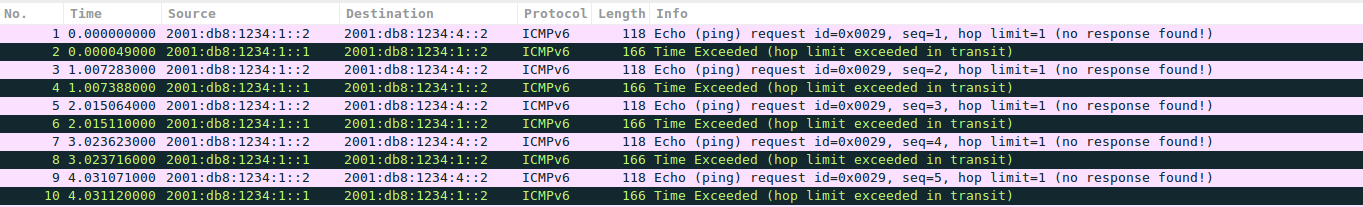
\includegraphics[width=0.95\textwidth]{ttl1.png}
        \caption{Captura del tráfico del ping entre n8 y n7.}
        \label{image:ttl1}
    \end{figure}

    \begin{figure}[H]
        \centering
        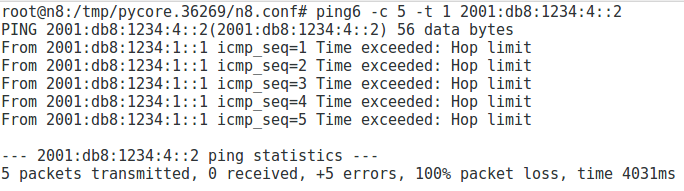
\includegraphics[width=0.75\textwidth]{ttl1ping.png}
        \caption{Salida del comando ping.}
        \label{image:ttl1ping}
    \end{figure}
\end{enumerate}

\section{Ejercicio 3}

\textit{Dual Stack}

\begin{enumerate}[a)]
    \item Configure en la parte “X” y en “B” la red en IPv4 e IPv6 en modo Dual Stack.
    
    Para configurar las partes "X" y "B" de la red, asignamos IPv4 a los host de cada red y a las interfaces del router.
    Para esto se asignan, e.g. IPv4 privadas de la clase A, aplicando VLSM sobre cada una de las partes. \\

    Dado el bloque IPv4, 10.0.0.0 (con mascara de subred 8 por ser la mascara de clase A), se necesitan IPs para 150 hosts en la Red X y 20 hosts para la Red B,
    quedando las siguientes IPv4 para cada una de las redes respectivamente: \\

    \begin{enumerate}[1.]
        \item Red X tiene asignada el bloque IPv4 10.0.0.0/24 con 254 hosts disponibles.
        \item Red B tiene asignada el bloque IPv4 10.0.1.0/27 con 30 hosts disponibles.
    \end{enumerate}

    Luego, quedan las siguientes IP de host,

    \begin{enumerate}[1.]
        \item Red X, router n3, eth2, 10.0.0.1/24
        \item Red X, host n10, eth0, 10.0.0.253/24
        \item Red X, host n12, eth0, 10.0.0.254/24
        \item Red B, router n3, eth3, 10.0.1.1/27
        \item Red B, host n15, eth0, 10.0.1.29/27 
        \item Red B, host dhcp-server, eth0, 10.0.1.30/27
    \end{enumerate}
    
    \item Genere tráfico IPv6 e IPv4 y compare.
    
    Analizando las capturas de las figuras \ref{image:ipv4} y \ref{image:ipv6} podemos observar la presencia del header offset en el tráfico de IPv4,
    que no se encuentra en las capturas de IPv6. A su vez, aparece el flag DF que en las capturas de IPv6 no está.
    El mismo nos indica la presencia de la Fragmentación. La \textbf{fragmentación IP} es un mecanismo que permite separar 
    \textit{(o fragmentar)} un paquete IP entre varios bloques de datos, si su tamaño sobrepasa la unidad 
    máxima de transferencia (Maximum Transfer Unit - MTU) del canal. \\

    Aunque el objetivo es una implementación para capas más altas (por ejemplo TCP/UDP) este no está conseguido en dos puntos:

    \begin{itemize}
        \item La fragmentación puede tener una gran influencia negativa en la actuación y en el flujo de datos.
        
        \item Si se pierde un fragmento, hay que retransmitir todos los fragmentos del paquete original. 
        Sin embargo IP no tiene mecanismos de seguridad o de timeout y es dependiente de las funciones de 
        seguridad de las capas más altas como TCP.        
    \end{itemize}

    Por las razones arriba mencionadas se intenta de evitar la fragmentación siempre que sea posible.

    En el caso de IPv6, IPv6 ya no permite a los routers fragmentar los paquetes. El emisor siempre está informado 
    con un mensaje ICMP cuando una fragmentación será necesaria. Así el emisor puede bajar su tamaño de paquete 
    para esta conexión y la fragmentación ya no es necesaria. En caso de requerirse una fragmentación; el host, es quien debe hacerla. \\
    
    \begin{figure}[H]
        \centering
        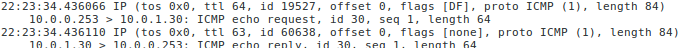
\includegraphics[width=0.95\textwidth]{ipv4.png}
        \caption{Ejemplo de tráfico en IPv4 capturado por tcpdump.}
        \label{image:ipv4}
    \end{figure}

    \begin{figure}[H]
        \centering
        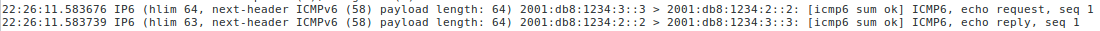
\includegraphics[width=0.95\textwidth]{ipv6.png}
        \caption{Ejemplo de tráfico en IPv6 capturado por tcpdump.}
        \label{image:ipv6}
    \end{figure}

    \item Investigue mecanismos para llevar el tráfico IPv4 de la red “X” a la red “B” pasando por redes. Vea cómo puede implementarse en la topología.

    Investigando otros mecanismos nos encontramos con el siguiente post: 
    \href{https://www.networkworld.com/article/2285078/tech-primers/ipv6--dual-stack-where-you-can--tunnel-where-you-must.html}{IPv6: Dual stack where you can; tunnel where you must}. \\

    En el mismo se describe como IPv6 se entregó con técnicas de migración para cubrir todos los casos de actualización de IPv4 
    concebibles, pero muchos fueron rechazados en última instancia por la comunidad tecnológica, y hoy nos queda un pequeño 
    conjunto de enfoques prácticos. \\

    Una técnica, llamada pila dual, implica ejecutar IPv4 e IPv6 al mismo tiempo. Los nodos finales y los enrutadores / conmutadores 
    ejecutan ambos protocolos, y si la comunicación IPv6 es posible, ese es el protocolo preferido. \\

    Otro enfoque es usar túneles para llevar un protocolo dentro de otro. Estos túneles toman paquetes de 
    IPv6 y los encapsulan en paquetes de IPv4 para enviarlos a través de partes de la red que aún no se han actualizado a IPv6. 
    Se pueden crear túneles donde haya islas IPv6 separadas por un océano IPv4, que será la norma durante las primeras 
    etapas de la transición a IPv6. Más adelante habrá islas IPv4 que deberán ser puenteadas a través de un océano IPv6. \\

    Otras técnicas, como la traducción de direcciones de red y la traducción de protocolos (NAT-PT) simplemente traducen los 
    paquetes IPv6 en paquetes IPv4. Estas técnicas de traducción son más complicadas que IPv4 NAT porque los protocolos tienen 
    diferentes formatos de encabezado. Las técnicas de traducción estaban destinadas a ser utilizadas como último recurso. \\

    El uso de técnicas de doble pila y tunelización es preferible al uso de NAT-PT.

\end{enumerate}

\end{document}
